\documentclass{cours}

\title{Loi Binomiale}

\begin{document}
    \maketitle{9}

    \begin{Gpartie}{Succession d'Épreuves Indépendantes} 
        \begin{Spartie}{Rappel} 
            Deux épreuves successives sont indépendantes lorsque le résultat de la première n'influe pas sur le résultat de la deuxième.

            \begin{center} % source https://texample.net/tikz/examples/probability-tree/
                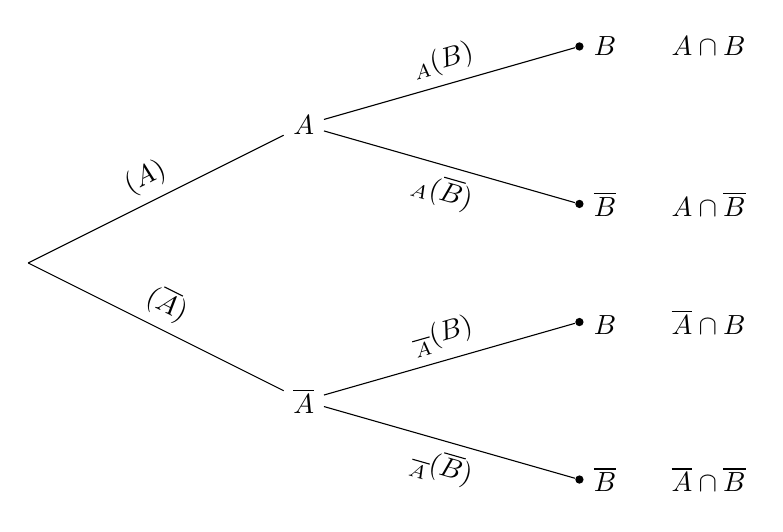
\begin{tikzpicture}[grow=right, sloped, scale=1]
                    \tikzstyle{level 1}=[level distance=3.5cm, sibling distance=3.5cm]
                    \tikzstyle{level 2}=[level distance=3.5cm, sibling distance=2cm]
                    \tikzstyle{end} = [circle, minimum width=3pt,fill, inner sep=0pt]
                    \coordinate
                        child {
                            node {$\overline{A}$}       
                                child {
                                    node[end, label=right:
                                        {$\overline{B}\qquad\overline{A}\cap\overline{B}$}] {}
                                    edge from parent
                                    node[below]  {$\Pde_{\overline{A}}(\overline{B})$}
                                }
                                child {
                                    node[end, label=right:
                                        {$B\qquad\overline{A}\cap B$}] {}
                                    edge from parent
                                    node[above] {$\Pde_{\overline{A}}({B})$}
                                }
                                edge from parent 
                                node[above] {$\Pde(\overline{A})$}
                        }
                        child {
                            node {$A$}        
                            child {
                                    node[end, label=right:
                                        {$\overline{B}\qquad A\cap\overline{B}$}] {}
                                    edge from parent
                                    node[below] {$\Pde_{A}(\overline{B})$}
                                }
                                child {
                                    node[end, label=right:
                                        {$B\qquad A\cap B$}] {}
                                    edge from parent
                                    node[above]  {$\Pde_{A}({B})$}
                                }
                            edge from parent         
                                node[above] {$\Pde(A)$}
                        };
                \end{tikzpicture}
                \parbox{\linewidth}{\captionof{figure}{Arbre de Probabilité qui Présente l'Indépendance des Épreuves}} \\[2ex]
            \end{center}
            Ainsi, $A$ et $B$ sont deux événements indépendants si et seulement si :
            \begin{itemize}
                \item $\Pde_A(B)=\Pde_{\overline{A}}(B)=\Pde(B)$
                \item $\Pde(A\cap B)=\Pde(A)\times\Pde(B)$
            \end{itemize}
        \end{Spartie}
        \pagebreak
        \begin{Spartie}{Modélisations} 
            On peut représenter une succession de $n$ épreuves indépendantes par un arbre pondéré (une issue de cette succession d'épreuves est alors un chemin sur l'arbre).

            Si les $n$ épreuves indépendantes ont pour univers respectifs $\Omega_1\,,\Omega_2\,,\dotsb\,,\Omega_n$, les issues de ces $n$ épreuves sont les éléments du produit cartésien $\Omega_1\times\Omega_2\times\dotsb\times\Omega_n$.
        \end{Spartie}
        \begin{Spartie}{Exemple} 
            Un restaurant propose deux entrées $e_1$ et $e_2$, trois plats $p_1$, $p_2$, et $p_3$ et un dessert $d$.

            Un client prend au hasard une entrée, un plat, et un dessert.

            L'ensemble des issues de cette expérience est $\Omega=\Omega_1\times\Omega_2\times\Omega_3$ où $\Omega_1=\big\{e_1\,; e_2\big\},~\Omega_2=\big\{p_1\,; p_2\,; p_3\big\},\text{ et }\Omega_3=\big\{d\big\}$.

            Ainsi, $\Omega=\bigg\{\big(e_1\,, p_1\,, d\big)\,;\big(e_1\,, p_2\,, d\big)\,;\dotsc\bigg\}$.

            On peut aussi représenter la situation par un arbre :
            \begin{center}
                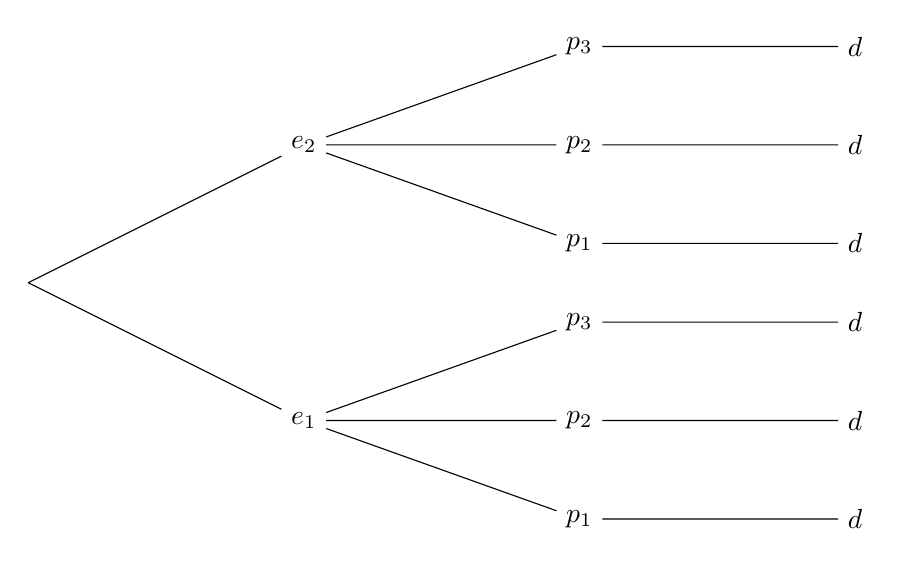
\begin{tikzpicture}[grow=right, sloped, scale=1]
                    \tikzstyle{level 1}=[level distance=3.5cm, sibling distance=3.5cm]
                    \tikzstyle{level 2}=[level distance=3.5cm, sibling distance=1.25cm]
                    \tikzstyle{level 3}=[level distance=3.5cm]
                    \tikzstyle{end} = [circle, minimum width=3pt,fill, inner sep=0pt]
                    \coordinate
                        child {
                            node {$e_1$}       
                                child {
                                    node {$p_1$} child { node {$d$} }
                                }
                                child {
                                    node {$p_2$} child { node {$d$} }
                                }
                                child {
                                    node {$p_3$} child { node {$d$} }
                                }
                        }
                        child {
                            node {$e_2$}        
                                child {
                                    node {$p_1$} child { node {$d$} }
                                }
                                child {
                                    node {$p_2$} child { node {$d$} }
                                }
                                child {
                                    node {$p_3$} child { node {$d$} }
                                }
                        };
                \end{tikzpicture}
                \parbox{\linewidth}{\captionof{figure}{Arbre Pondéré Représentant la Situation}}
                \\[2ex]
            \end{center}
        \end{Spartie}
    \end{Gpartie}
    \pagebreak
    \begin{Gpartie}{Loi Binomiale} 
        \vspace{-5ex}
        \begin{Spartie}{Épreuve de Bernoulli} 
            \vspace{-3ex}
            \begin{SSpartie}{Définition} 
                Une \emph{épreuve de} \textsc{Bernoulli} est un expérience aléatoire possédant deux issues qu'on appelle généralement \og succès \fg{} et \og échec \fg{}. La probabilité du succès $p$ est appelée paramètre de la loi de \textsc{Bernoulli}.
                \begin{center}
                    \begin{tabular}{  | p{0.1\textwidth} || *{2}{w{c}{0.1\textwidth} | }  } \hline
                        $k_i$           & $0$ & $1$ \\ \hline
                        $P(X=k_i)$      &$1-p$& $p$ \\ \hline
                    \end{tabular}
                    \parbox{\linewidth}{\captionof{figure}{Loi de la Variable Aléatoire X}}
                \end{center}
                $X$ est une variable aléatoire donnant le nombre de succès (il n'y a que deux possibilités : 0 ou 1). On dit que $X$ suit la loi de \textsc{Bernoulli}. \\ Penser à un jeu de pile ou face.
            \end{SSpartie}
            \begin{SSpartie}{Propriété} 
                Si $X$ est une variable aléatoire suivant la loi de \textsc{Bernoulli} de paramètre $p$, alors, l'espérance de $X$ est $E(X)=p$ et sa variance est $V(X)=p(1-p)$.
            \end{SSpartie}
        \end{Spartie}
        \begin{Spartie}{Schéma de Bernoulli} 
            \begin{SSpartie}{Définition} 
                Un \emph{schéma de} \textsc{Bernoulli} est une répétition de $n$ épreuves \emph{identiques} et \emph{indépendantes} à deux issues ($n$ épreuves de \textsc{Bernoulli}).

                Une issue de cette expérience aléatoire est un élément ($n$-uplet) de $\Omega=\big\{S\,;\overline{S}\big\}^n$.
            \end{SSpartie}
            \begin{SSpartie}{Exemple} 
                On tire successivement $4$ fois à pile ou face avec une pièce (truquée peut-être) dont la probabilité de tomber sur \og pile \fg{} est $p$. 
                
                Les tirages obtenus sont des 4-uplets composés de $P$ et de $F$ (si l'on note $P$ l'événement \og tomber sur pile \fg{} et $F$ \og tomber sur face \fg{}).
                
                Un exemple de tirage est $\big(P\,, F\,, F\,, F\big)$. On peut aussi noter $S$ et $\overline{S}$ au lieu de $P$ et $F$.
            \end{SSpartie}
        \end{Spartie}
        \pagebreak
        \begin{Spartie}{Loi Binomiale} 
            \begin{SSpartie}{Définition} 
                On considère une expérience aléatoire qui suit un schéma de \textsc{Bernoulli}, autrement dit, une répétition de $n$ épreuves \emph{identiques} et \emph{indépendantes} à deux issues (succès et échec) dont la probabilité de succès est $p$.

                La variable aléatoire donnant le nombre de succès suit la \emph{loi binomiale} de paramètres $n$ et $p$, notée $\mathcal{B}\,\left(n\,, p\right)$. Cette loi est aussi parfois appelée loi du nombre de succès.
            \end{SSpartie}
            \begin{SSpartie}{Propriété} 
                Soit $X$ une variable aléatoire suivant la loi binomiale de paramètres $n$ et $p$, on peut aussi noter $X\sim\mathcal{B}\,\left(n\,, p\right)$.

                Pour tout entier $k$ compris entre $0$ et $n$ :
                \[\boxed{P(X=k)=\binom{n}{k}p^k(1-p)^{n-k}}\]

                \begin{center}
                    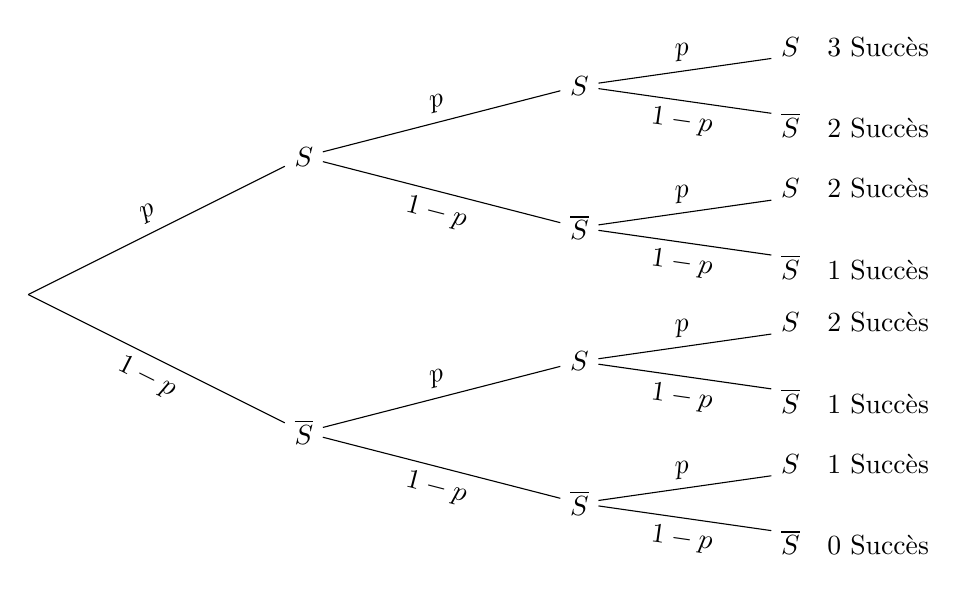
\begin{tikzpicture}[grow=right, sloped, scale=1]
                        \tikzstyle{level 1}=[level distance=3.5cm, sibling distance=3.5cm]
                        \tikzstyle{level 2}=[level distance=3.5cm, sibling distance=1.8cm]
                        \tikzstyle{level 3}=[level distance=3.5cm, sibling distance=1cm]
                        \tikzstyle{end} = [circle, minimum width=3pt,fill, inner sep=0pt]
                        \coordinate
                            child {
                                node {$\overline{S}$}        
                                    child {
                                        node {$\overline{S}$} 
                                            child {
                                                node {$\overline{S}$\quad 0 Succès}
                                                edge from parent node[below] {$1-p$}
                                            }
                                            child {
                                                node {$S$\quad 1 Succès}
                                                edge from parent node[above] {$p$}
                                            } 
                                        edge from parent node[below] {$1-p$}
                                    }
                                    child {
                                        node {$S$} 
                                            child {
                                                node {$\overline{S}$\quad 1 Succès}
                                                edge from parent node[below] {$1-p$}
                                            }
                                            child {
                                                node {$S$\quad 2 Succès}
                                                edge from parent node[above] {$p$}
                                            }
                                        edge from parent node[above] {$p$}
                                    }
                                edge from parent node[below] {$1-p$}
                            }
                            child {
                                node {$S$}        
                                    child {
                                        node {$\overline{S}$} 
                                            child {
                                                node {$\overline{S}$\quad 1 Succès}
                                                edge from parent node[below] {$1-p$}
                                            }
                                            child {
                                                node {$S$\quad 2 Succès}
                                                edge from parent node[above] {$p$}
                                            } 
                                        edge from parent node[below] {$1-p$}
                                    }
                                    child {
                                        node {$S$} 
                                            child {
                                                node {$\overline{S}$\quad 2 Succès}
                                                edge from parent node[below] {$1-p$}
                                            }
                                            child {
                                                node {$S$\quad 3 Succès}
                                                edge from parent node[above] {$p$}
                                            } 
                                        edge from parent node[above] {$p$}
                                    }
                                edge from parent node[above] {$p$}
                            };
                    \end{tikzpicture}
                        \parbox{\linewidth}{\captionof{figure}{Illustration de la Loi Binomiale}}
                \end{center}
                \pagebreak
                \begin{SSSpartie}{Démonstration} 
                    Dans l'arbre, chaque chemin contenant exactement $k$ succès passe par $k$ branches de probabilité $p$ et $n-k$ branches de probabilité $1-p$. Ainsi la probabilité d'un tel chemin est $p^k(1-p)^{n-k}$.

                    On compte ensuite le nombre de chemins contenant $k$ succès : il~y~en~a~$\binom{n}{k}$.

                    On peut aussi considérer qu'un tirage est un $n$-uplet contenant des $S$ et des $\overline{S}$.

                    Ainsi, un tirage contenant $k$ succès comporte $k$ fois la lettre $S$ et $n-k$ fois la lettre $\overline{S}$. Le nombre de façons de disposer les $k$ \og $S$ \fg{} parmi les $n$ éléments est $\binom{n}{k}$.
                \end{SSSpartie}
                \begin{SSSpartie}{Exemple} 
                    Avec nos $4$ tirages de pièce truquée, si on a $p=\frac{2}{3}$ (la probabilité de tirer \og pile \fg{} est $\frac{2}{3}$) et si on note $X$ la variable aléatoire donnant le nombre de \og pile \fg{}, on a :
                    \[P\big(X=1\big)=\binom{4}{1}\Bigg(\frac{2}{3}\Bigg)^1\Bigg(1-\frac{2}{3}\Bigg)^{4-1}=4\times\Bigg(\frac{2}{3}\Bigg)\times\Bigg(\frac{1}{3}\Bigg)^3\approx 0{,}099\]
                \end{SSSpartie}
            \end{SSpartie}
            \begin{SSpartie}{Propriété} 
                Soit $X$ une variable aléatoire suivant la loi binomiale $\mathcal{B}\,\left(n\,, p\right)$.

                L'Espérance de $X$ est $\boxed{E(X)=np}$. \\ La variance de $X$ est $\boxed{V(X)=np(1-p)}$. \\ L'Écart-type de $X$ est $\boxed{\sigma(X)=\sqrt{np(1-p)}}$.

                Démonstration dans chapitre sur les opérations sur les Variables Aléatoires.
                \begin{SSSpartie}{Exemple} 
                    On reprend la pièce truquée précédente, qu'on lance quatre fois. $X$ est toujours la variable aléatoire donnant le nombre de \og pile \fg.

                    $E(X)=4\times\frac{2}{3}\approx 2{,}67$\quad (On peut espérer d'obtenir 2{,}67 piles sur 4 tirages)

                    $\sigma(X)=\sqrt{4\times\frac{2}{3}\times\frac{1}{3}}\approx 0{,}94$\quad (Dont l'interprétation est moins intéressante)
                \end{SSSpartie}
            \end{SSpartie}
        \end{Spartie}
    \end{Gpartie}
\end{document}